\chapter{Introduction}
\label{sec:Introduction}

A distinct problem arising from attempting to study the exact state of sea ice is that there is limited data available. Data pertaining to sea ice is widely distributed, not correlated, or limited in scope such that it's difficult to draw inferences from. Naturally, the immediate approach to this thesis will first require research into available data sources before conducting any exploration. Exploration of these sources will reveal which sources should be targeted for the remainder of the thesis.
\\
\indent After reviewing the preliminary research, this paper will move forward to a more targeted effort in obtaining and analyzing data to develop a machine learning model. Chapter 2 will describe the process of obtaining the selected data, and Chapter 3 will discuss the methodology of developing the model.
------------
\\
Provide a general introduction to what the thesis is all about. Here you present the question or problem you aim to answer or address with your thesis, some of the reasons why it is a worthwhile topic, what has been done in prior work and where the gap is that the thesis addresses.

\section{Preliminary Research}
Preliminary research into the availability of ice thickness data yields two notable organizations which may act as sources of data. These two organizations are the National Snow and Ice Data Center (NSIDC), and the National Aeronautics and Space Administration (NASA). Although both organizations offer large amounts of data, they differ in approach. The NSIDC acts as a historic repository, accumulating previous studies into a single location for easy access. NASA offers a similar service, but additionally allows researchers the opportuntity to query information from any of their active orbitting satellites.
/// Add the European Space Agency as another portal - as this will be discussed in preliminary exploration. If not, it will surely need to be discussed somewhere, including the process of retrieving it, because it's the data set we're using for the model.  ////

\subsection*{NASA}
Here is where you should include sources to the ATL10 Data Specification pdf, and the associated CryoSat data specs. It should also be included where these links came from. It also should be included where, if applicable, specific data downloads were from. It should include the process of querying for data, which portals are made accessible, and how flexible they are. Do not forget to mention that they made an IceSat-2 mobile application for iOS.

Include how NASA's Sentinel-2 delivers SAR imaging, but at 50m resolution. This is a modality that can be used for a CNN but the resolution is not meaningfully compatible with any source of ground truth we have. Thus, searching for alternatives led to the European Space Agency and its sponsorship for ICEYE's 1m resolution imaging.

Somewhere you should discuss IceSat-2 and its laser altimetry. ESPECIALLY that it's 17m footprint offers precision at a given location, 
\subsection*{NSIDC}
Here is where the NSIDC links and data retrieval should be discussed. Limitations of the data or other notes about it's composition should be included according to the details in the abstract saved on file. Preliminary exploration will be where the figures will be uploaded (Or maybe we show one figure showing all of the points, and the exploration will be for the single instance?)

\section {Preliminary Exploration}
Data of interest were the IceSat-2 ATL10 product and the NSIDC In-situ Dataset, selected for their combination of breadth and accuracy. Furthermore, the European Space Agency's requirements for sponsored data need to be explored to pursue the higher resolution SAR imagery hoped for. //
After preliminary exploration, NASA's IceSat-2 satellite and the NSIDC's "On-Ice Arctic Sea Ice Thickness Measurements by Auger, Core, and Electromagnetic Induction, from the Late 1800s Onward, Version 2" dataset appeared to be the most promising sources of truth for the study. The in-situ measurements would be invaluable in developing a basic understanding of how ice actually is, while the laser altimetry appears to be second-most accurate, especially in consideration of the availability of data it offers.
\subsection*{NASA}
A single delivery of IceSat-2's ATL10 data product yields a '.h5' file, incompatibile with traditional spreadsheets. To access IceSat-2 data in a meaningful way, involved developing a script to extract relevant information according to the types enumerated in the data product specificiation. Columns of interest include the latitude, longitude, time, and calculated freeboard height for each of the three beam pairs.
\subsection*{NSIDC}
The "On-Ice Arctic Sea Ice Thickness Measurements by Auger, Core, and Electromagnetic Induction, from the Late 1800s Onward, Version 2" contains 69,750 rows of data, spanning 5 categorized regions; the Arctic Ocean, the Beaufort Sea, Greenland Coast, Prudhoe Bay, and Russian Coast. Filtering down to the Beaufort Sea region, a region of interest, yields 23 separate studies ranging between 1958 to 2016.
\begin{figure}[h]
	\centering
	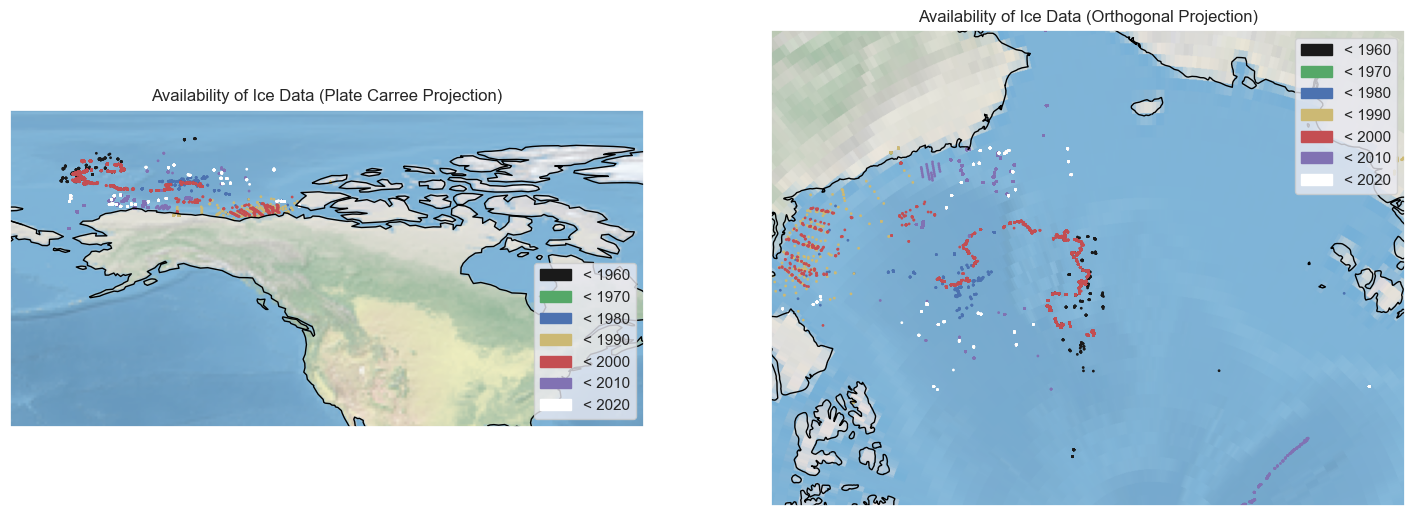
\includegraphics[width=\linewidth]{../research-resources/in-situ/Plotted-Tracks.png}
	\caption{Beaufort Sea In-Situ Studies}
	\label{fig:bfsea-in-situ-agg}
\end{figure}

For a simple analysis, the largest single dataset was chosen to conduct a simple test on the distribution of sea ice thickness. This distribution if normal will reasonably allow for future condicting of statistical tests, and if not normal will give insight as to what a reasonable assumption of ice thickness distribution should be. The following data set is composed of 21,547 distinct points which would intuitively capture the simple patterns that are hoped to be extracted.

\begin{figure}[h]
	\centering
	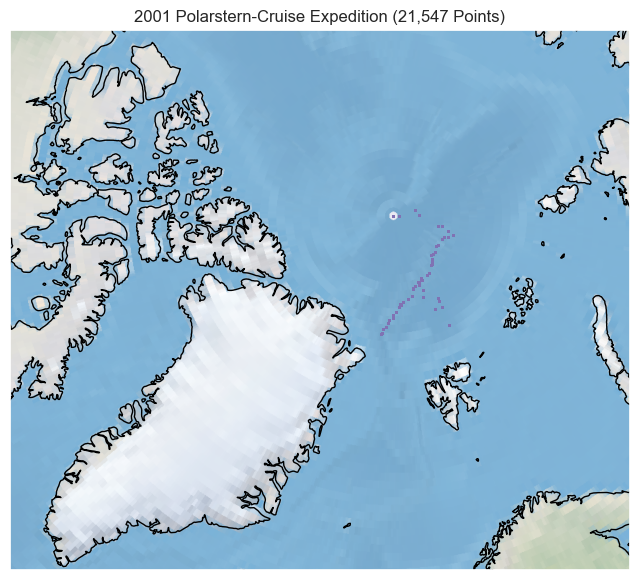
\includegraphics[width=.8\linewidth]{../research-resources/in-situ/region-of-interest.png}
	\caption{}
	\label{fig:bfsea-in-situ-spec}
\end{figure}